\section{The Constant-Depth Carry-Save Technique}
\label{sec:csa}

Our 2D factoring approach rests on the central technique of the constant-depth
carry-save adder (CSA) \cite{Gossett1998}, which converts the sum of three
numbers $a$, $b$, and $c$, to the sum of two numbers $u$ and $v$:
%\begin{equation}
$a+b+c = u+v$. The explanation of this technique and how it achieves constant depth requires the following definitions.
%\end{equation}

A \emph{conventional number} $x$ can be represented in $n$ bits as
%\begin{equation}
$x = \sum_{i=0}^{n-1} 2^i x_i$,
%\end{equation}
where $x_i \in \{0,1\}$ denotes the $i$-th bit of $x$, which we call
an $i$-bit and has significance $2^i$, and the $0$-th bit is the low-order bit.\footnote{It will be clear from the context whether we mean an
$i$-bit, which has significance $2^i$, or an $i$-bit number.}
Equivalently, $x$ can be represented as a (non-unique)
sum of two smaller, $(n-1)$-bit, conventional numbers, $u$ and $v$.
We say $(u+v)$ is a \emph{carry-save encoded}, or CSE, number.
The CSE representation of an $n$-bit conventional number
consists of $2n-2$ individual
bits where $v_0$ is always $0$ by convention.

Consider a CSA operating on three bits instead of three numbers; 
then a CSA converts the sum of three
$i$-bits into the sum of an $i$-bit (the \emph{sum} bit) and an $(i+1)$-bit
(the \emph{carry} bit):
%\begin{equation}
%\label{eqn:csa-3-2}
$a_i+b_i+c_i = u_i+v_{i+1}$.
%\end{equation}
By convention, the bit $u_i$ is the parity of the input bits
($u_i = a_i \oplus b_i \oplus c_i$) and
the bit $v_{i+1}$ is the majority of $\{a_i, b_i, c_i\}$.
Figure \ref{fig:csa-encoding} gives a concrete example, where
$(u+v)$ has $2n-2 = 8$ bits, not counting $v_0$.

%
It will also be useful to refer to a subset of the bits in a conventional
number using subscripts to indicate a range of indices:
\begin{equation}
x_{(j,k)} \equiv \sum_{i=j}^k 2^ix_i \qquad
x_{(i)} \equiv x_{(i,i)} = 2^ix_i.
\end{equation}
%
Using this notation, the following identity holds:
\begin{equation}
x_{(j,k)} = x_{(j,\ell)} + x_{(\ell+1,k)}, \qquad \text{ for all } j \le \ell < k.
\end{equation}
%
We can express the relationship between the bits of $x$ and $(u+v)$ as follows:
%
\begin{equation}
x = x_{(0,n-1)} \equiv u+v = u_{(0,n-2)} + v_{(1,n-1)}.
\end{equation}
%
Finally, we denote arithmetic modulo $m$ with square brackets.

\begin{equation}
x_{(j,k)} \bmod m = x_{(j,k)}[m]
\end{equation}

\begin{center}
\begin{figure*}[tb!]
\begin{displaymath}
x = 30 = u+v = 8 + 22 = \left\{
\begin{array}{ccccc}
    & u_3 & u_2 & u_1 & u_0 \\
v_4 & v_3 & v_2 & v_1 &    \\
\hline
x_4 & x_3 & x_2 & x_1 & x_0
\end{array}
\right\}
=
\left\{
\begin{array}{ccccc}
    & 1 & 0 & 0 & 0 \\
  1 & 0 & 1 & 1 &   \\
\hline
1 & 1 & 1 & 1 & 0
\end{array}
\right\}
\end{displaymath}
\caption{An example of carry-save encoding for the 5-bit conventional number 30.}
\label{fig:csa-encoding}
\end{figure*}
\end{center}
%

\begin{figure}[tb!]
\begin{center}
\begin{displaymath}
\centerline{
\Qcircuit @C=2em @R=2em {
\lstick{\ket{0}}   & \qw      & \qw & \qw                        & \qw & \qw                        & \targfix  & \qw & \qw_{\ket{a_i \wedge (b_i \oplus c_i)}} & \targfix  & \qw       & \qw       & \qw_{\ket{(b_i \wedge c_i) \oplus a_i \wedge (b_i \oplus c_i)}} & \qw & \qswap      & \qswap      & \qw & \rstick{\ket{u_i}} \\
\lstick{\ket{a_i}} & \qw      & \qw & \qw                        & \qw & \qw                        & \ctrl{-1} & \qw & \qw                                     & \qw       & \targfix  & \qw       & \qw_{\ket{a_i \oplus b_i \oplus c_i}}                           & \qw & \qw \qwx    & \qswap \qwx & \qw & \rstick{\ket{0}} \\
\lstick{\ket{b_i}} & \ctrl{1} & \qw & \targfix                   & \qw & \qw_{\ket{b_i \oplus c_i}} & \ctrl{-1} & \qw & \qw                                     & \qw       & \ctrl{-1} & \targfix  & \ctrl{1}                                                        & \qw & \qw \qwx    & \qw         & \qw & \rstick{\ket{b_i}} \\
\lstick{\ket{c_i}} & \ctrl{1} & \qw & \ctrl{-1}                  & \qw & \qw                        & \qw       & \qw & \qw                                     & \qw       & \qw       & \ctrl{-1} & \ctrl{1}                                                        & \qw & \qw \qwx    & \qw         & \qw & \rstick{\ket{c_i}} \\
\lstick{\ket{0}}   & \targfix & \qw & \qw_{\ket{b_i \wedge c_i}} & \qw & \qw                        & \qw       & \qw & \qw                                     & \ctrl{-4} & \qw       & \qw       & \targfix                                                        & \qw & \qswap \qwx & \qw         & \qw & \rstick{\ket{v_{i+1}}}}
}
\end{displaymath}
\caption{Carry-save adder circuit for a single bit position $i$: $a_i+b_i+c_i = u_i + v_{i+1}$.}
\label{fig:csa-circuit}
\end{center}\end{figure}

\begin{figure}
\begin{center}
\begin{displaymath}
\begin{tabular}{p{0.5in} m{0.1in} p{2in}}

\Qcircuit @C=1em @R=2.2em { 
	& \qw & \ctrl{1} & \qw & \qw \\
	& \qw & \ctrl{1} & \qw & \qw \\
	& \qw & \targfix & \qw & \qw
}

&
\qquad
=
\qquad
&

\Qcircuit @C=1em @R=.7em { 
	& \gate{T^{\dagger}} & \qw & \targfix  & \qw & \gate{T} & \qw & \targfix  & \qw & \gate{T^{\dagger}} & \qw & \targfix  & \qw & \gate{T}           & \qw & \targfix  & \qw & \qw \\ 
	& \gate{T^{\dagger}} & \qw & \qw       & \qw & \ctrl{1} & \qw & \ctrl{-1} & \qw & \ctrl{1}           & \qw & \qw       & \qw & \qw                & \qw & \ctrl{-1} & \qw & \qw \\
	& \gate{H}           & \qw & \ctrl{-2} & \qw & \targfix & \qw & \gate{T}  & \qw & \targfix           & \qw & \ctrl{-2} & \qw & \gate{T^{\dagger}} & \qw & \gate{H}  & \qw & \qw
}
\end{tabular}
\end{displaymath}
\caption{The depth-efficient Toffoli gate decomposition from \cite{Amy2012}.}
\label{fig:toffoli}
\end{center}
\end{figure}

% From Notebook #16, pp. 68-69
\begin{table}
\begin{displaymath}
\begin{tabular}{|c|c|c|c|}
\hline
\text{Circuit Name} & \text{Depth} & \text{Size} & \text{Width} \\
\hline
\text{Toffoli gate from \cite{Amy2012}} and Figure \ref{fig:toffoli} & 8 & 15 & 3 \\
\hline
\text{Single-bit } 3\text{-to-}2 \text{ adder from Figure \ref{fig:csa-circuit}} & 33 & 55 & 5 \\
%\hline
%$n$ \text{-bit modular } 3\text{-to-}2 \text{ adder from Figure \ref{fig:csa-add-4}} & 356 & 572n + 724 & 33n+47 \\
\hline
\end{tabular}
\end{displaymath}
\centerline{}
\caption{Circuit resources for Toffoli and single-bit addition.}
\label{tab:csa-tile-resources}
\end{table}

Figure \ref{fig:csa-circuit} gives a circuit description of carry-save addition (CSA) for a single bit position $i$.
The resources for this circuit are given in Table \ref{tab:csa-tile-resources}, using
the resources for the Toffoli gate (in the same table) based on
\cite{Amy2012}. We note here
that a more efficient decomposition for the Toffoli is possible using a
distillation approach described in \cite{Jones2013a}.

We must lay out the circuit to satisfy a 2D NTC model.
The Toffoli gate decomposition in \cite{Amy2012}, duplicated in
Figure \ref{fig:toffoli}, requires two control
qubits and a single target qubit to be
mutually connected to each other. Given this constraint, and the
interaction of the CNOTs in Figure \ref{fig:csa-circuit}, we can
rearrange these qubits on a 2D planar grid and obtain the layout shown
in Figure \ref{fig:csa-3-2}, which satisfies our 2D NTC model.
Qubits $\ket a_i$, $\ket b_i$, and $\ket c_i$ reside at the top of Figure~\ref{fig:csa-3-2}, while qubits $\ket{u_i}$ and $\ket{v_{i+1}}$ are initialized to $\ket 0$.
Upon completion of the circuit, qubit $\ket{a_i}$ is in state $\ket 0$, as seen from the output in Figure~\ref{fig:csa-circuit}. 
Note that this construction uses more gates and one more ancilla than the equivalent
quantum full adder circuit in Figure 5 of \cite{Gossett1998}. However this
is necessary in order to meet our architectural constraints and does not change the
asymptotic results.
Also in Figure \ref{fig:csa-3-2}
is a variation called a 2-2 adder, which simply re-encodes two $i$-bits
into an $i$-bit and an $(i+1)$-bit. The 2-2 adder uses at most the resources
of a 3-2 adder, so we can count it as such in our calculations.
It will be useful in the next section.

\begin{figure}[b!]
\begin{center}
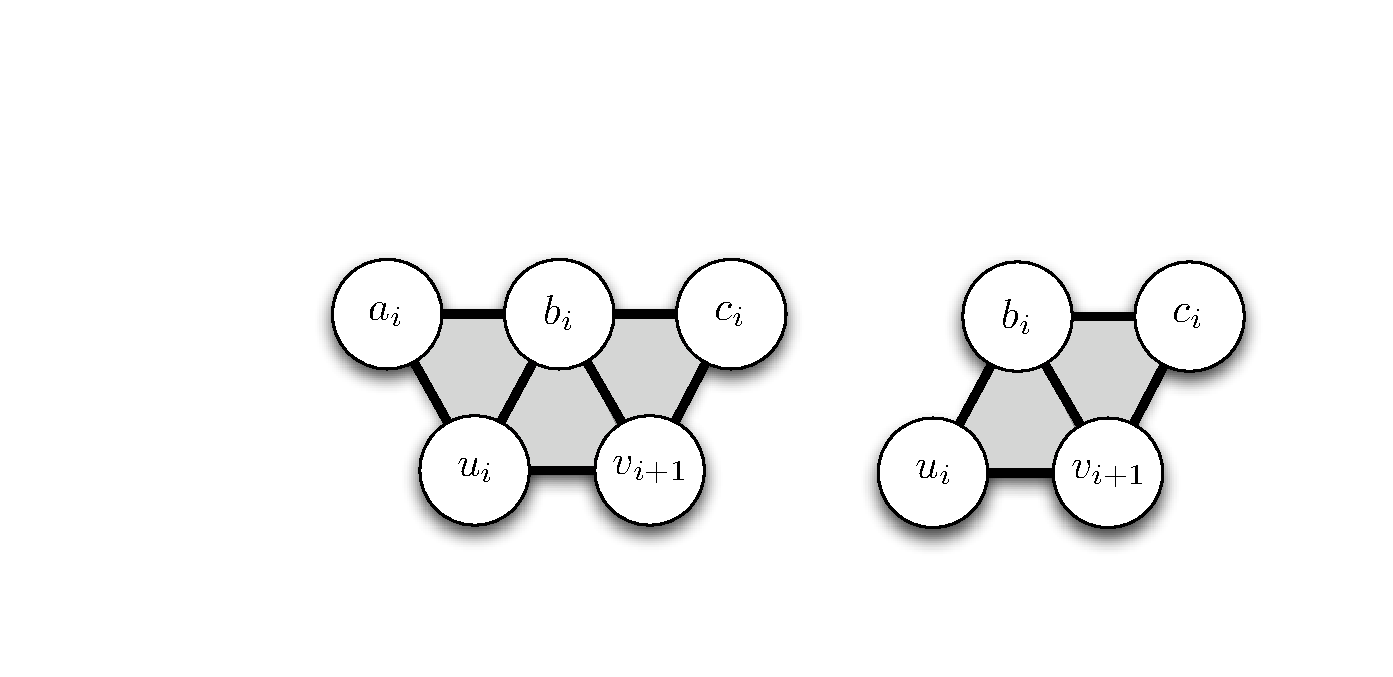
\includegraphics[width=3in]{factor-polylog/figures/csa-32-22.pdf}
\end{center}
\caption{The carry-save adder (CSA), or 3-2 adder, and carry-save 2-2 adder.}
\label{fig:csa-3-2}
\end{figure}

At the level of numbers, the sum of three $n$-bit numbers can be converted into
the sum of two $n$-bit numbers by applying a \emph{CSA layer} of
$n$ parallel, single-bit
CSA circuits (Fig.~\ref{fig:csa-circuit}). Since each CSA operates in constant depth, the entire layer also
operates in constant depth, and we have achieved (non-modular) addition.
%
%An important consideration is the circuit width. The circuit above
%requires two additional qubits to contain the output
%out-of-place and produces two garbage qubits: the original inputs
%$b_i$ and $c_i$. 
Each single addition of three $n$-bit numbers requires $O(n)$ circuit width.